Chimera states have been observed in many other systems, whether they be purely mathematical, biological, electrical, or mechanical [\onlinecite{Shanahan2010,Abrams2004,Andrzejak2016,Hizanidis2016,Kuramoto2002,Martens2013,Panaggio2015,Santos2015,Santos2017,Kruk2018,Xie2014}].
One of the most common ways that chimera states are talked about is in regards to seizures.

\subsubsection{Neuroanatomy and Neurophysiology}
\label{sec:intro_seizures_neuroanatomy}
Since the brain is an electrochemical device, its function and disorders are often best talked about from an electrical standpoint [\onlinecite{Deco2008}].
Neurons are cells which are specialized for communication (see \cref{fig:neuron_diagram} for a diagram).
\begin{figure}[ht]
  \centering
  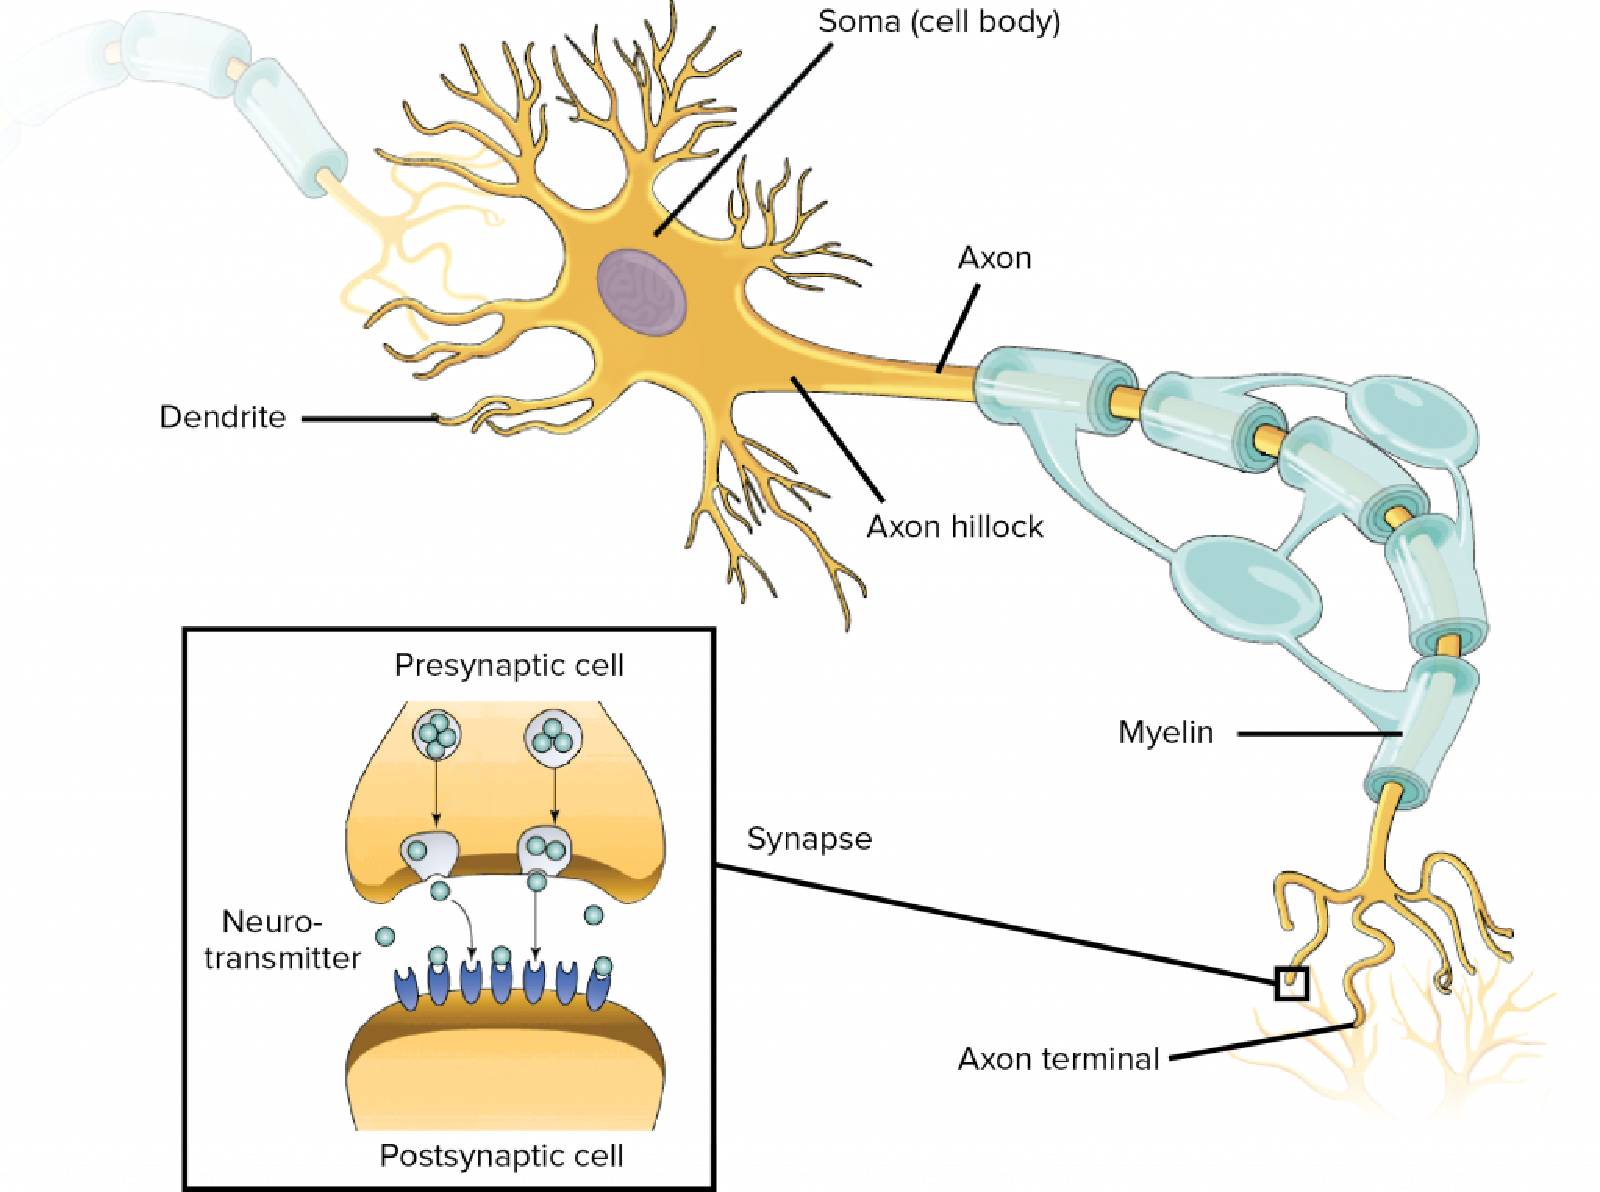
\includegraphics[width=0.8\columnwidth]{figure/neuron_diagram.pdf}
  \caption[Neuron diagram]{A diagram of the anatomy of a neuron.
    Taken from [\onlinecite{Molnar2013}] on a \href{https://creativecommons.org/licenses/by/4.0/}{CC BY 4.0 license}.
  }
  \label{fig:neuron_diagram}
\end{figure}
They receive input signals through synapses at the ends of their dendrites, branches in their large tree of inputs.
The trunk of the dendritic tree is the soma, the cell body.
If the sum signal entering the soma from all of the dendrites is sufficient, the neuron fires, sending a signal to its outputs.

When a neuron fires, it sends an electrochemical signal down its axon---its long stem---to the output synapses at its axon terminals.
This signal is known as an action potential.
The action potential is discrete; a neuron sends the same signal any time its input threshold is surpassed, no matter how far above the threshold the input is.
It is the propagation along the axon of a potential difference across the cell membrane of the neuron.
This potential difference is created by different concentrations of various ions in and out of the cell, controlled by pumps (which push \ce{Na^{+}} out of the cell and draw \ce{K^{+}} into it) and gates (which allow the ion concentrations to equilibrate).
It is important to note that processes involving \ce{Na^{+}} are faster than those involving \ce{K^{+}}.
Each location along the axon goes through the following six stages, in total taking approximately \SI{1}{\ms}:
\begin{description}
\item[Equilibrium] No current flows through the membrane, which has a potential of \SI{-75}{\mV} across it\footnote{All potentials hold the extracellular matrix at \SI{0}{\V}.  In other words, the interior of the cell is at a lower potential than the exterior.}.

\item[Depolarization] The potential difference propagating from upstream in the axon activates ion channel gates, allowing \ce{Na^{+}} to flow into the axon, countered by the \ce{K^{+}} flowing out.

\item[Amplification] Because the \ce{K^{+}} processes are slower than the \ce{Na^{+}} processes, if the incoming signal is strong enough, the influx of \ce{Na^{+}} is too fast for the outflow of \ce{K^{+}} to compensate.
  This results in a positive feedback loop, wherein the \ce{Na^{+}} flowing in increases the membrane potential, which increases the rate at which \ce{Na^{+}} flows into the neuron, which continues to feed itself.

\item[Repolarization] When the \ce{Na^{+}} channels are fully open, the \ce{K^{+}} channels are finally able to compensate for the influx.

\item[Hyper-polarization] The \ce{Na^{+}} channels close, and the slower \ce{K^{+}} channels remain open.
  This causes more \ce{K^{+}} to flow out of the cell than \ce{Na^{+}} flowed in, dropping the potential below its equilibrium state.

\item[Refractory Period] The \ce{Na^{+}} channels are briefly unable to open, which means that neurons need a brief time to ``recharge'' after an action potential.

\end{description}

%% \subsubsubsection{Micro-scale models}
All of these processes are summarized in the Hodgkin-Huxley model\footnote{A full derivation of this model can be found in [\onlinecite{Graben2008}].} describing the membrane potential $U$:
\begin{multline}
  \label{eq:hodgkin_huxley_main}
  C_{m} \dot{U}
  +
  p_{A \ce{K^{+}}} \mean{g}_{A \ce{K^{+}}} \pqty{U - E_{\ce{K^{+}}}} \\
  +
  p_{A \ce{Na^{+}}} \mean{g}_{A \ce{Na^{+}}} \pqty{U - E_{\ce{Na^{+}}}}
  +
  g_{l} \pqty{U - E_{l}}
  =
  I_{m}
\end{multline}
where
\begin{equation}
  \label{eq:hodgkin_huxley_supplementary}
  \begin{aligned}
    \dot{n}
    &=
    \alpha_{n} \pqty{1 - n} \beta_{n} n, \\
    \dot{m}
    &=
    \alpha_{m} \pqty{1 - m} \beta_{m} m, \\
    \dot{h}
    &=
    \alpha_{h} \pqty{1 - h} \beta_{h} h,
  \end{aligned}
  \qand
  \begin{aligned}
    p_{A \ce{K^{+}}}
    &=
    n^{4}, \\
    p_{A \ce{Na^{+}}}
    &=
    m^{3} h.
  \end{aligned}
\end{equation}
where $g_{i}$ is the conductance of the membrane to ion $i$, $p_{A i}$ is the proportion of $i$-gates which are open (developed from a Markov model with transition rates $\alpha$ and $\beta$), $E_{i}$ is the equilibrium potential of ion $i$, $C_{m}$ is the capacitance of the membrane, and $I_{m}$ is an external current (the tuned input parameter).
This model is highly accurate, and won its developers a Nobel Prize in Physiology or Medicine.
Many bifurcation analyses have been performed on these equations, and they are well understood [\onlinecite{Graben2008}].

However, the Hodgkin-Huxley model is not particularly useful for large-scale brain simulation.
Given that most behavior of the brain is emergent\footnote{One of the classic ways to explain emergence is asking, ``Where is the thought in a neuron?''}, it is important to understand neurons' interactions.
As is often the case with emergent phenomena, it is wildly impractical to simulate the collective behavior of a brain by simulating its constituent neurons.
Since the human brain has approximately $10^{11}$ neurons with $10^{14}$ synapses, direct simulation is too computationally intensive.
To better understand the dynamics of large portions of the brain, many researchers have turned to the techniques of thermal and statistical physics [\onlinecite{Breakspear2017}],
resulting in \textit{neural ensemble models} and \textit{neural mass models} as two popular approaches to studying brain behavior.

%% \subsubsubsection{Meso-scale Models}
%% \label{sec:intro_seizures_neuroanatomy_meso_scale}
Neural ensemble models treat patches of the brain as a collective group, taking into account neurons' mean activity, as well as their variance.
They assume that the firings of the neurons within a group are sufficiently uncorrelated to result in a Gaussian distribution of firing rates.
This means that the behavior of the ensemble is linear, even though the behavior of the constituent neurons is highly nonlinear.
One can then use a Fokker-Planck equation to describe the collective dynamics of the population.
The main benefit to these models is that they are well-studied in fields like solid-state physics.
However, recent work has shown that the assumption of Gaussian firing rates is not accurate [\onlinecite{Breakspear2017}].
Firing rates do tend to fall into well-behaved distributions, but not ones that lend themselves to already-developed tools.

For higher coherence within populations (i.e., a non-Gaussian distribution of firing rates), researchers tend to use neural mass models.
They assume that nearby neurons in the brain are sufficiently synchronized to model groups of them as a single neuron, with some modifications.
Instead of the discrete action potential of a single neuron, neural mass models often have a sigmoidal activation function.
Researchers also simplify the dynamics of the Hodgkin-Huxley model to divide the neural mass's constituent neurons into two subpopulations: an excitatory pool (corresponding to the \ce{Na^{+}} channels in the Hodgkin-Huxley model) and an inhibitory pool (corresponding to the \ce{K^{+}} channels in the Hodgkin-Huxley model).

An example of a neural mass model is the extremely simple Wilson-Cowan model [\onlinecite{Wang2012}]:
\begin{align}
  \label{eq:wc_x}
  \tau_{x} \dot{x}
  &=
    -x + S \pqty{C_{x x} x + C_{x y} y + C_{x z} z + P}, \\
  \label{eq:wc_y}
  \tau_{y} \dot{y}
  &=
    -y + S \pqty{C_{y x} x + C_{y y} y + C_{y z} z + Q},
\end{align}
and
\begin{equation}
  \label{eq:wc_z}
  \tau_{z} \dot{z}
  =
    -z + S \pqty{C_{z x} x + C_{z y} y + C_{z z} z + R}.
\end{equation}
Here, $x$ represents an excitatory process (like the flow of \ce{Na^{+}}), and $y$ and $z$ represent inhibitory processes (like the flow of \ce{K^{+}}).
The time constants $\tau_{i}$ determine the rates of the dynamics of the three processes.
It is worth noting that chaotic dynamics can occur when multiple different time scales are present [\onlinecite{Breakspear2017}].
The coupling strengths $C_{i j}$ represent the connectivity between the three processes, with $C_{i x} \geq 0$ (making $x$ excitatory) and $C_{i \Bqty{y, z}} \leq 0$ (making $y$ inhibitory).
$P$, $Q$, and $R$ represent the excitability threshold, or the constant external inputs to each process (similar to $I_{m}$ in \cref{eq:hodgkin_huxley_main}).
The sigmoidal activation function $S(x) = \frac{1}{1 + e^{-a \pqty{x - \theta}}}$ represents the mass effect of the population of neurons being modeled.
This system provides an excellent toy model which reflects meso-scale dynamics accurately, relative to its simplicity.

%% \subsubsubsection{Macro-scale Models}
%% \label{sec:intro_seizures_neuroanatomy_macro_scale}
These two models do an accurate job of representing the behavior of small parts of the brain.
However, it is not reasonable to carry the assumptions of un- or highly-correlated activity to the large-scale activity of whole-brain dynamics.
To make these models more accurately depict the overall behavior of the brain as a whole, researchers turn to two main techniques: neural field models and neural mass networks.
The first treats the brain as a continuous sheet of cortex, within which activity obeys wave equations.
The second represents the brain as a discrete graph of cortices, or a network of coupled oscillators.
The network used for the coupling of the oscillators is determined by the brain's connectivity matrix, or connectome.
An example of a neural mass network model is the modified Hindmarsh-Rose model [\cref{eq:hr_x,eq:hr_y,eq:hr_z}], which we discuss later.

One of the benefits of a neural mass network model is that its outputs are similar to those of an electroencephalograph, or EEG.
The EEG is a device used to record the electrical activity of the brain.
Electrodes are placed in specific areas on the scalp, and then changes in voltage are measured from neural masses beneath the skull.
Much of the signal is distorted and attenuated by the bone and tissue between the brain and the electrodes, which act like resistors and capacitors.
This means that, while the membrane voltage of the neuron changes by millivolts, the EEG reads a signal in the microvolt scale [\onlinecite{Kandel2013}].
The EEG also has relatively low spatial and temporal resolution (16 electrodes for the whole brain, and a sampling rate of \SI{33}{\ms}).
However, when properly treated, neural mass models make for effective predictors of the output from EEGs [\onlinecite{Taylor2012,Leistritz2007}].
This is useful, as EEGs are the main tool used to detect and categorize seizures.

\subsubsection{Seizure \AE tiology}
\label{sec:intro_seizures_aetiology}
For centuries, and across many cultures, seizures were viewed as holy and mystical events, and those with epilepsy were in many cases believed to be shamans [\onlinecite{Kandel2013,Fadiman1998}].
Seizures are often accompanied by strange visions, sounds, or smells (called auras), and sometimes manifest themselves physically in extreme ways.
External symptoms can include convulsions of the limbs or the entire body, or a seeming trance.
In societies that are unfamiliar with the root causes of seizures, this can be a terrifying and awe-inspiring sight to behold.

In more recent years, researchers have come to define seizures as abnormal, excessive, or overly-synchronized neural activity [\onlinecite{Kandel2013,Baier2012}].
It is important to distinguish between seizures and epilepsy, as the two are often conflated.
Seizures are an acute event, whereas epilepsy is a chronic condition of repeated seizures.
While classification schemes vary, all center around the division between generalized and focal seizures.

Generalized seizures involve the entire brain, and start in both hemispheres at the same time, which is why they are often called primary generalized seizures.
The manifestation of these seizures crosses an entire spectrum.
They sometimes hardly present to an external observer, as in the case of the typical absence seizure\footnote{Due to early epilepsy research being performed in French-speaking regions, ``absence'' is pronounced \textipa{\ae b"sAns}.}, which is nonconvulsive and results in a complete cessation of motor activity for approximately 10 seconds.
Patients lose consciousness, but not posture, making it seem to an observer like a trance or simply ``spacing out.''

On the other side of the range is the tonic-clonic seizure, wherein effectively all of a patient's muscles contract at once for around 30 seconds (the tonic phase), and then clench and unclench rapidly, resulting in jerking of the extremities (the clonic phase) for 1 to 2 minutes.
After tonic-clonic seizures (in the postictal phase), patients often report confusion, muscle soreness, and exhaustion.

Focal seizures start in one part of the brain (the seizure focus).
They are generally preceded by auras such as a sense of fear, or hearing music, and often manifest as clonic movement of the extremities.
In many cases, they secondarily generalize, spreading to the entire brain.
This can make focal seizures and primary generalized seizures hard to distinguish, as a focal seizure can generalize rapidly after a brief aura.
This can lead to misdiagnoses and improper treatments.

%% \subsubsubsection{The Epileptor Model}
%% \label{sec:intro_seizures_aetiology_epileptor}
An empirical/phenomenological seizure model called Epileptor was recently developed by Jirsa \etal [\onlinecite{Jirsa2014,Jirsa2017}].
The model involves two fast processes $x_{1}$ and $y_{1}$, two spike-wave event processes $x_{2}$ and $y_{2}$, and a slow permittivity variable $z$.
Its guiding equations are:
\begin{align}
  \label{eq:epileptor_x1}
  \dot{x}_{1}
  ={}&
    y_{1}
    -
    f_{1}(x_{1}, x_{2})
    -
    z
    +
    I_{\text{rest} 1}, \\
  \label{eq:epileptor_y1}
  \dot{y}_{1}
  ={}&
    y_{0}
    -
    5 x_{1}^{2}
    -
    y_{1}, \\
  \label{eq:epileptor_z}
  \dot{z}
  ={}&
    \frac{1}{\tau_{0}} \pqty{4 \pqty{x_{1} - x_{0}} - z}, \\
  \label{eq:epileptor_x2}
  \dot{x}_{2}
  ={}&
    -y_{2}
    +
    x_{2}
    -
    x_{2}^{3}
    +
    I_{\text{rest} 2} \\
    &{}\quad +
    0.002 g(x_{1})
    -
    0.3 \pqty{z - 3.5}, \\
  \label{eq:epileptor_y2}
  \dot{y}_{2}
  ={}&
    \frac{1}{\tau_{2}} \pqty{-y_{2} + f_{2}(x_{1}, x_{2})},
\end{align}
where
\begin{align}
  \label{eq:epileptor_g}
  g(x_{1})
  ={}&
    \int_{t_{0}}^{t}{e^{-\gamma \pqty{t - \tau}} x_{1}(\tau) \dd{\tau}}, \\
  \label{eq:epileptor_f1}
  f_{1}(x_{1}, x_{2})
  ={}&
    \begin{cases}
      x_{1}^{3} - 3 x_{1}^{2}
      \text{ if } x_{1} < 0, \\
      x_{1} \pqty{x_{2} - 0.6 \pqty{z - 4}^{2}}
      \text{ if }
      x_{1} \geq 0,
    \end{cases}
\end{align}
and
\begin{equation}
  \label{eq:epileptor_f2}
  f_{2}(x_{1}, x_{2})
  =
    \begin{cases}
      0
      \text{ if } x_{2} < -0.25, \\
      6 \pqty{x_{2} + 0.25}
      \text{ if } x_{2} \geq -0.25.
    \end{cases}
\end{equation}
The required parameters have the following values: $x_{0} = -1.6$, $y_{0} = 1$, $\tau_{0} = 2857$, $\tau_{1} = 1$, $\tau_{2} = 10$, $I_{\text{rest} 1} = 3.1$, $I_{\text{rest} 2} = 0.45$, and $\gamma = 0.01$.
A feature to note is that $\tau_{0} \gg \tau_{2} \gg \tau_{1}$.
As previously mentioned, these vastly different time scales allow for chaotic dynamics to occur, and contribute to the nonlinearity of the system.

While the Epileptor model is highly accurate, and is currently being used to develop patient-specific models and treatments, its main issue is that it is purely phenomenological and not fully rooted in theory.
EEG traces of humans, mice, and zebrafish were collected, and parameters were adjusted until $x_{1} + x_{2}$ matched the measured traces, resulting in the above values.
The model may be an important tool for treating symptoms, but is not necessarily as valuable for determining root causes.

%%% Local Variables:
%%% mode: latex
%%% TeX-master: "../../ms"
%%% End:
